% !TeX program = xelatex
% 高一数学 · 4.2.1 指数函数的概念
% 编译：xelatex 指数函数的概念.tex（连续两遍）
\documentclass[aspectratio=169,11pt,t,fleqn]{ctexbeamer}

\usepackage{amsmath,amssymb}
\usepackage{tabularx}% 自动调整表格宽度
\usepackage{booktabs}% 制作专业的三线表 提供了\toprule（顶线）、\midrule（中线）和 \bottomrule底线命令。
\usepackage{graphicx}% 插入与处理图形 它的核心命令是 \includegraphics。
\usepackage{multirow}% 合并多行单元格 负责表格的纵向结构，实现跨行合并。 提供了 \multirow 命令
\usepackage{colortbl}
\usepackage{caption}
\captionsetup[figure]{name=图}
\setbeamertemplate{caption}[numbered] % 图形自动编号
\linespread{1.2}% 修改全文行距
\usepackage{pgfplots}
\pgfplotsset{compat=1.18}

% ---- 思源字体 ----
\setCJKmainfont{Source Han Serif SC}[BoldFont={Source Han Serif SC Bold}]
\setCJKsansfont{Source Han Sans SC}[BoldFont={Source Han Sans SC Bold}]
\usefonttheme[stillsansseriflarge]{serif}
% ---- 配色（教材蓝）----
\definecolor{mainblue}{RGB}{23,103,171}
\definecolor{lightblue}{RGB}{222,235,247}
\definecolor{accent}{RGB}{196,60,50}
\definecolor{dotpink}{RGB}{214,60,120}

\definecolor{xyyg}{cmyk}{0,1,1,0.45}%{rgb}{0.543,0.0,0.0703} %{cmyk}{0,100,100,45}%{rgb}{0.5,0.0,0.0}  %RGB#820010
\definecolor{xyyg_gold}{cmyk}{0,0.35,0.75,0.05}
\definecolor{xyyg_blue}{cmyk}{0.6,0.35,0.0,0.4}
\definecolor{xyyg_darkblue}{cmyk}{1.0,0.6,0.0,0.5}
\definecolor{xyyg_gray}{cmyk}{0.0,0.0,0.08,0.55}
\definecolor{xyyg_dirt}{cmyk}{0.0,0.2,0.35,0.3}

\setbeamertemplate{theorems}[numbered]% 定理自动编号
\newtheorem{instance}{例}% 新建例题环境
\BeforeBeginEnvironment{instance}{% 
	\setbeamercolor{block title}{bg=xyyg_darkblue,fg=white}
	\setbeamercolor{block body}{bg=xyyg_blue!10}
}
\AfterEndEnvironment{instance}{
	\setbeamercolor{block title}{bg=xyyg,fg=white}
	\setbeamercolor{block body}{bg=xyyg!10}
}


%\useoutertheme[subsection=false]{smoothbars}
\usetheme{Boadilla}
%\usetheme{Singapore}
\usecolortheme{whale}
%\usecolortheme{spruce}
\setbeamercolor{structure}{fg=xyyg}
\setbeamercolor{alerted text}{fg=accent}

\setbeamercolor{palette primary}{use=structure,fg=white,bg=structure.fg}
\setbeamercolor{palette secondary}{use=structure,fg=white,bg=structure.fg!70!black}
\setbeamercolor{palette tertiary}{use=structure,fg=white,bg=structure.fg!20!black}
\setbeamercolor{palette quaternary}{fg=white,bg=structure.fg!85!black}

\AtBeginDocument{
% 设置 alertblock 标题栏的颜色（fg=前景色，bg=背景色）
\setbeamercolor{block title alerted}{fg=white, bg=structure.fg!80}
% 设置 alertblock 正文区域的颜色
\setbeamercolor{block body alerted}{fg=black, bg=structure!10}
% 设置 exampleblock 标题栏颜色
\setbeamercolor{block title example}{fg=white, bg=green!50!black}
% 设置 exampleblock 正文区域颜色
\setbeamercolor{block body example}{fg=black, bg=green!10}

\setbeamercolor{block title}{bg=xyyg,fg=white}
\setbeamercolor{block body}{bg=xyyg!10}

\setbeamertemplate{enumerate items}[default]
\setbeamertemplate{itemize items}[ball]
}


% 散点 + 趋势线通用样式（x 为距 2001 年的偏移年，刻度映射回年份）
\pgfplotsset{
	scenic/.style={
		clip=false,
		width=8cm, height=6cm,
		xmin=0, xmax=14.7, ymin=100, ymax=1600,
		xtick={0,2,4,6,8,10,12,14},
		xticklabels={2001,2003,2005,2007,2009,2011,2013,2015},
		ytick={300,500,700,900,1100,1300},
		xlabel={年份}, ylabel={人次/万次},
		axis lines=center,
		label style={font=\small},
		%    ylabel style={left},
		xlabel style={above},
		tick label style={font=\footnotesize, /pgf/number format/1000 sep={}},
		xticklabel style={rotate=30, anchor=east,xshift=5pt,yshift=-3pt},
		%    enlargelimits=0.03,
	},
}
\usepackage[most]{tcolorbox}
\tcbuselibrary{,}
\newtcolorbox{summarybox}[1][]{
	colback=purple!10,enhanced, drop fuzzy shadow=gray,
	colframe=purple!70!black,
	fonttitle=\bfseries,
	title=#1,
	arc=1mm,
	boxrule=0pt,
	left=2mm, right=2mm, top=2mm, bottom=2mm,
}


\title[指数函数的概念]{4.2 指数函数}
\subtitle{4.2.1 指数函数的概念}
\author[好好学习，努力向上]{}
\date{2026-11-21}

\begin{document}

% ============ 标题页 ============
\begin{frame}
  \titlepage
\end{frame}

% ============ 复习引入 ============
\begin{frame}{复习引入}
  对于幂 $a^x$（$a>0$），我们已经把指数 $x$ 的范围拓展到了实数。上一章学习了函数的概念和基本性质，通过对幂函数的研究，进一步了解了研究一类函数的过程和方法。

  \vspace{1em}
  下面继续研究其他类型的基本初等函数。
\end{frame}

% ============ 问题 1（情境文字）============
\section{问题一}
\begin{frame}{问题情景}
  \begin{block}{问题 1}
    随着中国经济高速增长，人民生活水平不断提高，旅游成了越来越多家庭的重要生活方式。由于旅游人数不断增加，A、B 两地景区自 2001 年起采取了不同的应对措施，A 地提高了景区门票价格，而 B 地则取消了景区门票。

    \vspace{0.5em}
    表 4.2-1 给出了 A、B 两地景区 2001 年至 2015 年的游客人次以及逐年增加量。
  \end{block}
\end{frame}

% ============ 问题 1 数据表 4.2-1 ============
\begin{frame}[t]{表 4.2-1\quad A、B 两地景区游客人次及逐年增加量}
  \centering\vspace{-1em}
  \begin{columns}
  	\column{0.3\textwidth} 
  	 \begin{itemize}
  		\item 比较两地景区游客人次的变化情况，你发现了怎样的变化规律？
  		\item<2-> 为了有利于观察规律，根据表 4.2-1，分别画出 A、B 两地景区采取不同措施后的 15 年游客人次的图象（图 4.2-1 和图 4.2-2）。
  	\end{itemize}
  	
  	
  	\column{0.69\textwidth}
  	  \scriptsize
  	\renewcommand{\arraystretch}{1.15}
  	\begin{tabular}[t]{|c|c|c|c|c|}
  		\hline
  		\rowcolor{xyyg!60}
  		\multirow[c]{2}{*}{\cellcolor{xyyg!70} } &
  		\multicolumn{2}{c|}{\textbf{A 地景区}} &
  		\multicolumn{2}{c|}{\textbf{B 地景区}} \\
  		\cline{2-5}
  		\rowcolor{xyyg!50}
  		\cellcolor{xyyg!70}\textbf{时间/年}  & \textbf{人次/万次} & \textbf{年增加量/万次} & \textbf{人次/万次} & \textbf{年增加量/万次} \\
  		\hline
  		2001 & 600 & — & 278 & — \\
  		\hline
  		2002 & 609 & 9 & 309 & 31 \\
  		\hline
  		2003 & 620 & 11 & 344 & 35 \\
  		\hline
  		2004 & 631 & 11 & 383 & 39 \\
  		\hline
  		2005 & 641 & 10 & 427 & 44 \\
  		\hline
  		2006 & 650 & 9 & 475 & 48 \\
  		\hline
  		2007 & 661 & 11 & 528 & 53 \\
  		\hline
  		2008 & 671 & 10 & 588 & 60 \\
  		\hline
  		2009 & 681 & 10 & 655 & 67 \\
  		\hline
  		2010 & 691 & 10 & 729 & 74 \\
  		\hline
  		2011 & 702 & 11 & 811 & 82 \\
  		\hline
  		2012 & 711 & 9 & 903 & 92 \\
  		\hline
  		2013 & 721 & 10 & 1005 & 102 \\
  		\hline
  		2014 & 732 & 11 & 1118 & 113 \\
  		\hline
  		2015 & 743 & 11 & 1244 & 126 \\
  		\hline
  	\end{tabular}
  \end{columns}

%  \multicolumn{cols}{pos}{text}是原生命令
%  \multirow[vpos]{number of rows}{width or *}{text}来自multyrow宏包
  
\end{frame}



% ============ 问题 1 图象：图 4.2-1 / 4.2-2 ============
\begin{frame}{问题 1\quad 两地景区游客人次图象}
  \begin{columns}
    \column{0.5\textwidth}
    \centering
    \begin{tikzpicture}
      \begin{axis}[scenic]
        \addplot[only marks, mark=*, dotpink, mark size=2pt] coordinates {
          (0,600) (1,609) (2,620) (3,631) (4,641)
          (5,650) (6,661) (7,671) (8,681) (9,691)
          (10,702) (11,711) (12,721) (13,732) (14,743)
        };
        \addplot[xyyg, dashed, thick, domain=0:14] {600 + 10.21*x};
      \end{axis}
    \end{tikzpicture}\\[2pt]
    图 4.2-1\quad A 地景区（线性增长）

    \column{0.5\textwidth}
    \centering
    \begin{tikzpicture}
      \begin{axis}[scenic,]
        \addplot[only marks, mark=*, dotpink, mark size=2pt] coordinates {
          (0,278) (1,309) (2,344) (3,383) (4,427)
          (5,475) (6,528) (7,588) (8,655) (9,729)
          (10,811) (11,903) (12,1005) (13,1118) (14,1244)
        };
        \addplot[xyyg, dashed, thick, domain=0:14] {278*1.11^x};
      \end{axis}
    \end{tikzpicture}\\[2pt]
    图 4.2-2\quad B 地景区（指数增长）
  \end{columns}
\end{frame}

% ============ 问题 1 观察比较 ============
\begin{frame}{问题 1\quad 观察与比较}
	
	
	\vspace{0.8em}
	\begin{block}{观察图象和表格，可以发现}
		\begin{itemize}
			\item A 地景区的游客人次近似于直线上升（\alert{线性增长}），年增加量大致相等（约为 10 万次）；
			\item B 地景区的游客人次则是\alert{非线性增长}，年增加量越来越大，但从图象和年增加量都难以看出变化规律。
		\end{itemize}
	\end{block}
\end{frame}

% ============ 问题 1 探究：增长率 ============
\begin{frame}{问题 1\quad 探究：年增长率}
  \begin{block}{探究}
    年增加量是对相邻两年的游客人次做减法得到的。能否通过对 B 地景区每年的游客人次做其他运算发现游客人次的变化规律呢？
  \end{block}
\pause
  从 2002 年起，将 B 地景区每年的游客人次除以上一年的游客人次，可以得到
  \[
    \frac{2002\text{ 年游客人次}}{2001\text{ 年游客人次}}=\frac{309}{278}\approx 1.11,\qquad
    \frac{2003\text{ 年游客人次}}{2002\text{ 年游客人次}}=\frac{344}{309}\approx 1.11,
    \]
  \[
    \cdots\cdots,\qquad
    \frac{2015\text{ 年游客人次}}{2014\text{ 年游客人次}}=\frac{1244}{1118}\approx 1.11.
  \]

  结果表明，B 地景区游客人次的\alert{年增长率}都约为 $1.11-1=0.11$，是一个常数。像这样，增长率为常数的变化方式，我们称为\alert{指数增长}。
\end{frame}

% ============ 问题 1 指数增长模型 ============
\begin{frame}{问题 1\quad 指数增长模型}
  从 2001 年开始，B 地景区游客人次的变化规律可以近似描述为：
  \begin{itemize}
    \item 1 年后，游客人次是 2001 年的 $1.11^1$ 倍；
    \item 2 年后，游客人次是 2001 年的 $1.11^2$ 倍；
    \item 3 年后，游客人次是 2001 年的 $1.11^3$ 倍；
    \item $\cdots\cdots$
    \item $x$ 年后，游客人次是 2001 年的 $1.11^x$ 倍。
  \end{itemize}

  \vspace{0.6em}
  如果设经过 $x$ 年后的游客人次为 2001 年的 $y$ 倍，那么
  \[
    y=1.11^x\qquad (x\in[0,+\infty)). \tag{1}
  \]
  这是一个函数，其中指数 $x$ 是自变量。
\end{frame}

% ============ 问题 2（文字与推导）============
\section{问题二}
\begin{frame}{}
  \small
  \begin{block}{问题 2}
    当生物死亡后，它机体内原有的碳 14 含量会按确定的比率衰减（称为衰减率），大约每经过 $5\,730$ 年衰减为原来的一半，这个时间称为“半衰期”。按照上述变化规律，生物体内碳 14 含量与死亡年数之间有怎样的关系？
  \end{block}
\pause
  设死亡生物体内碳 14 含量的年衰减率为 $p$，如果把刚死亡时的含量看成 1 个单位，那么
  \begin{align*}
    \setlength{\jot}{3pt}
    \text{死亡 1 年后，含量为 }&(1-p)^1;\\
    \text{死亡 2 年后，含量为 }&(1-p)^2;\\
    \text{死亡 3 年后，含量为 }&(1-p)^3;\\
    &\cdots\cdots\\
    \text{死亡 }5\,730\text{ 年后，含量为 }&(1-p)^{5730}.
  \end{align*}
  根据已知条件，$(1-p)^{5730}=\dfrac12$，从而 $1-p=\left(\dfrac12\right)^{\frac1{5730}}$，所以
  $p=1-\left(\dfrac12\right)^{\frac1{5730}}$。
\end{frame}

% ============ 问题 2 指数衰减模型 ============
\begin{frame}{问题 2\quad 指数衰减模型}
  设生物死亡年数为 $x$，死亡生物体内碳 14 含量为 $y$，那么 $y=(1-p)^x$，即
  \[
    y=\left(\left(\frac12\right)^{\frac1{5730}}\right)^x\qquad (x\in[0,+\infty)). \tag{2}
  \]

  \vspace{0.5em}
  这也是一个函数，指数 $x$ 是自变量。死亡生物体内碳 14 含量每年都以
  $1-\left(\dfrac12\right)^{\frac1{5730}}$ 的衰减率衰减。像这样，衰减率为常数的变化方式，我们称为\alert{指数衰减}。因此，死亡生物体内碳 14 含量呈指数衰减。
\end{frame}

% ============ 指数函数的概念 ============
\section{指数函数的概念}
\begin{frame}{指数函数的概念}
  如果用字母 $a$ 代替上述 (1)(2) 两式中的底数 $1.11$ 和 $\left(\dfrac12\right)^{\frac1{5730}}$，那么函数 $y=1.11^x$ 和 $y=\left(\left(\dfrac12\right)^{\frac1{5730}}\right)^x$ 就可以表示为
  \[
    y=a^x
  \]
  的形式，其中指数 $x$ 是自变量，底数 $a$ 是一个大于 $0$ 且不等于 $1$ 的常量。

  \vspace{0.8em}\pause
  \begin{alertblock}{定义}
    一般地，函数 $\textcolor{accent}{y=a^x\ (a>0,\ \text{且 }a\neq 1)}$ 叫做\alert{指数函数}（exponential function），其中指数 $x$ 是自变量，定义域是 $\mathbb{R}$。
  \end{alertblock}
\end{frame}

% ============ 例 1 ============
\section{例题分析}
\begin{frame}{}
  \begin{instance}
  	已知指数函数 $f(x)=a^x$（$a>0$，且 $a\neq 1$），且 $f(3)=\pi$，求 $f(0)$，$f(1)$，$f(-3)$ 的值。
  \end{instance}

  \vspace{0.5em}
  %\textbf{分析：}要求 $f(0)$，$f(1)$，$f(-3)$ 的值，应先求出 $f(x)=a^x$ 的解析式，即先求 $a$ 的值。
\pause
  \vspace{0.5em}
  \textbf{解：}因为 $f(x)=a^x$，且 $f(3)=\pi$，则 $a^3=\pi$，解得 $a=\pi^{\frac13}$，于是
  \[
    f(x)=\pi^{\frac{x}{3}}.
  \]
  所以，
  \[
    f(0)=\pi^0=1,\qquad
    f(1)=\pi^{\frac13}=\sqrt[3]{\pi},\qquad
    f(-3)=\pi^{-1}=\frac1\pi.
  \]
\end{frame}

% ============ 例 2 ============
\begin{frame}{}\vspace{-1em}
\begin{instance}
  \begin{enumerate}[(\arabic*)]
    \item 在问题 $1$ 中，如果平均每位游客出游一次可给当地带来 $1\,000$ 元门票之外的收入，A 地景区的门票价格为 $150$ 元，比较这 $15$ 年间 A、B 两地旅游收入变化情况。
    \item 在问题 $2$ 中，某生物死亡 $10\,000$ 年后，它体内碳 $14$ 的含量衰减为原来的百分之几？
  \end{enumerate}
\end{instance}
  \vspace{0.4em}\pause
  \textbf{解：}(1) 设经过 $x$ 年，游客给 A、B 两地带来的收入分别为 $f(x)$ 和 $g(x)$，则
  \[
    f(x)=1150\times(10x+600),\qquad
    g(x)=1000\times278\times1.11^x.
  \]
  利用计算工具可得：当 $x=0$ 时，$f(0)-g(0)=412\,000$；当 $x\approx10.22$ 时，$f(10.22)\approx g(10.22)$。结合图象可知：当 $x<10.22$ 时，$f(x)>g(x)$；当 $x>10.22$ 时，$f(x)<g(x)$；当 $x=14$ 时，$g(14)-f(14)\approx347\,303$。

  \vspace{0.4em}
  (2) 设生物死亡 $x$ 年后，它体内碳 14 含量为 $h(x)$。把刚死亡时的含量看成 1 个单位，则
  $h(x)=\left(\left(\dfrac12\right)^{\frac1{5730}}\right)^x$。当 $x=10\,000$ 时，
  $h(10\,000)=\left(\dfrac12\right)^{\frac{10000}{5730}}\approx0.30$，即衰减为原来的约 $30\%$。
\end{frame}

% ============ 图 4.2-3 收入对比 ============
\begin{frame}{例 2(1)\quad 两地旅游收入变化（图 \ref{fig:lvyou}）}
  \centering
  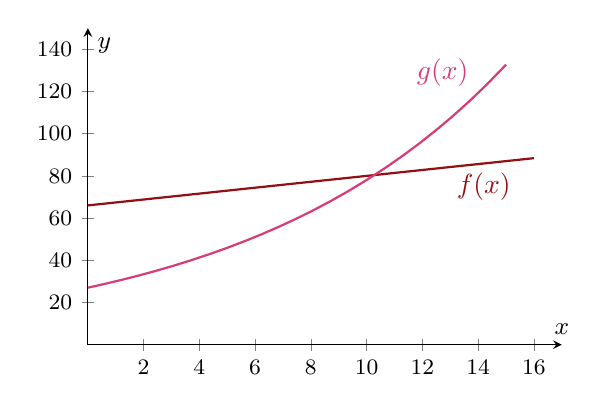
\begin{tikzpicture}
    \begin{axis}[
      width=7.6cm, height=5.6cm,
      xmin=0, xmax=17, ymin=0, ymax=150,
      xtick={0,2,4,6,8,10,12,14,16}, ytick={20,40,60,80,100,120,140},
      xlabel={$x$}, ylabel={$y$},
      axis lines=center,
      label style={font=\small},
      xlabel style={above},
      tick label style={font=\footnotesize},
%      enlargelimits=0.03,
    ]
      \addplot[xyyg, thick, domain=0:16] {66 + 1.4*x};
      \node[xyyg, anchor=north] at (axis cs:14.2,86) {$f(x)$};
      \addplot[dotpink, thick, domain=0:15] {27*1.112^x};
      \node[dotpink, anchor=south east] at (axis cs:14,118) {$g(x)$};
    \end{axis}
  \end{tikzpicture}
	\captionof{figure}{}\label{fig:lvyou}
\end{frame}

% ============ 指数增长 / 衰减模型 ============
\begin{frame}{常用函数模型}
  在实际问题中，经常会遇到类似于例 2(1) 的指数增长模型：设原有量为 $N$，每次的增长率为 $p$，经过 $x$ 次增长，该量增长到 $y$，则
  \[
    y=N(1+p)^x\quad (x\in\mathbb{N}).
  \]

  \vspace{0.6em}
  形如
  \[
   \boxed{\alert{ y=k a^x }\quad (k\in\mathbb{R},\ \text{且 }k\neq0;\ a>0,\ \text{且 }a\neq1)\rule[10pt]{0pt}{2pt}\rule[-5pt]{0pt}{2pt}}
  \]
  的函数是刻画指数增长或指数衰减变化规律的非常有用的函数模型。
\end{frame}

% ============ 小结 与 作业 ===========

\begin{frame}{}
	\begin{block}{小结：}
		\begin{enumerate}[(1)]
			\item 指数函数的概念\quad 形如$ y = a^x (a > 0, \text{且} a \neq 1) $这样的函数叫做指数函数。
			\item 指数函数模型 \quad 形如 $ y = k a^x (k \in \mathbb{R}, k \neq 0 , a > 0 ,\text{且} a \neq 1) $的函数。
		\end{enumerate}
	\end{block}
\end{frame}

\begin{frame}{布置作业}
	\begin{summarybox}[作业：]
		\begin{enumerate}[(1)]
			\item P115 练习1、2、3
			\item P118---119 习题4.2\quad 1、2.
		\end{enumerate}
	\end{summarybox}
\end{frame}

% ============ 练习 1（图象选项）============
\begin{frame}{练习 1}
  下列图象中，有可能表示指数函数的是（\quad ）。

  \vspace{0.6em}
  \pgfplotsset{
    opt/.style={
      width=4.0cm, height=4.0cm,
      axis lines=middle, axis equal,
      xtick=\empty, ytick=\empty,
      xmin=-2, xmax=2, ymin=-2.5, ymax=2.5,
      every axis plot/.append style={xyyg, thick},
      samples=100,
      xlabel={$x$},
      ylabel={$y$},
      ylabel style={left},
      xlabel style={below},
    },
  }
  \begin{columns}
    \column{0.25\textwidth}
    \centering
    \begin{tikzpicture}
      \begin{axis}[opt]
        \addplot[domain=-1.6:1.8] {-x+1.3};
        \node[below left] at (axis cs:0,0) {$O$};
      \end{axis}
    \end{tikzpicture}\\[2pt] (A)
    \column{0.25\textwidth}
    \centering
    \begin{tikzpicture}
      \begin{axis}[opt]
        \addplot[domain=-1.8:1.8] {x^2-2};
        \node[below left] at (axis cs:0,0) {$O$};
      \end{axis}
    \end{tikzpicture}\\[2pt] (B)
    \column{0.25\textwidth}
    \centering
    \begin{tikzpicture}
      \begin{axis}[opt]
        \addplot[domain=-2:1.7] {2^x};
        \node[below left] at (axis cs:0,0) {$O$};
      \end{axis}
    \end{tikzpicture}\\[2pt] (C)
    \column{0.25\textwidth}
    \centering
    \begin{tikzpicture}
      \begin{axis}[opt]
        \addplot[domain=-1.5:1.5] {x^3};
        \node[below right] at (axis cs:0,0) {$O$};
      \end{axis}
    \end{tikzpicture}\\[2pt] (D)
  \end{columns}
\end{frame}

\begin{frame}[t]{4.2.1 练习 第1题 解答}\vspace{-1em}
	\begin{tcolorbox}[colback=xyyg!10,colframe=xyyg!90,title=\textbf{解}]
		指数函数 $y=a^{x}\ (a>0,a\ne 1)$ 必满足：
		\begin{itemize}
			\item 定义域为 $\mathbf{R}$，图象向左右两方无限延伸；
			\item 图象恒过定点 $(0,1)$，即 $x=0$ 时 $y=1$；
			\item 当 $a>1$ 时单调递增，当 $0<a<1$ 时单调递减；
			\item 函数值恒为正，图象在 $x$ 轴上方。
		\end{itemize}
		
		\vspace{0.4em}
		(A) 是直线（一次函数）；(B) 是抛物线（二次函数）；
		(D) 图象过原点 $(0,0)$，不满足过 $(0,1)$。只有 (C) 是递增且过 $(0,1)$ 的曲线。
		
		\vspace{0.4em}
		\textbf{答案：C。}
	\end{tcolorbox}
\end{frame}


% ============ 练习 ============
\begin{frame}{练习}
  \begin{enumerate}
    \setcounter{enumi}{1}
    \item 已知函数 $y=f(x)$，$x\in\mathbb{R}$，且 $f(0)=3$，
      $\dfrac{f(0.5)}{f(0)}=2$，$\dfrac{f(1)}{f(0.5)}=2$，$\cdots$，
      $\dfrac{f(0.5n)}{f(0.5(n-1))}=2$，$n\in\mathbb{N}^*$，求函数 $y=f(x)$ 的一个解析式。
    \item 在某个时期，某湖泊中的蓝藻每天以 $6.25\%$ 的增长率呈指数增长，那么经过 30 天，该湖泊的蓝藻会变为原来的多少倍？（可以使用计算工具）
  \end{enumerate}
\end{frame}

\begin{frame}[t]{4.2.1 练习 第2题 解答}\vspace{-1em}
	\begin{tcolorbox}[colback=xyyg!10,colframe=xyyg!90,title=\textbf{解:}]
		由题意，自变量每增加 $0.5$，函数值就变为原来的 $2$ 倍，即
		\[
		f(x+0.5)=2\,f(x).
		\]
		设 $f(x)=3a^{x}$（由 $f(0)=3$ 得系数为 $3$），则
		\[
		f(x+0.5)=3a^{x+0.5}=a^{0.5}\cdot 3a^{x}=a^{0.5}f(x)=2f(x),
		\]
		故 $a^{0.5}=2$，解得 $a=4$。
		
		所以
		$
		\alert{f(x)=3\cdot 4^{x}=3\cdot 2^{2x}}.
		$
		
		\small（验证：$f(0)=3,\ f(0.5)=3\cdot 2=6,\ f(1)=12$，相邻两项之比均为 $2$，符合题意。）
	\end{tcolorbox}
\end{frame}

\begin{frame}[t]{4.2.1 练习 第3题 解答}\vspace{-1em}\vspace{-0.5em}
	\linespread{1.0}\selectfont
	\begin{tcolorbox}[colback=xyyg!10,colframe=xyyg!90,title=\textbf{解}]
		设原有蓝藻量为 $N_{0}$，经过 $x$ 天后蓝藻量为
		\[
		N(x)=N_{0}(1+6.25\%)^{x}=N_{0}\cdot 1.0625^{x}.
		\]
		当 $x=30$ 时，
		\[
		N(30)=N_{0}\cdot 1.0625^{30}.
		\]
		用计算工具：
		\[
		1.0625^{30}\approx 6.13.
		\]
		所以经过 $30$ 天，该湖泊的蓝藻约变为原来的 $\alert{6.13}$ 倍。
	\end{tcolorbox}
\end{frame}

\end{document}
